\chapter{The theory behind the Milky Way}

\section{Preliminary calculations}

Let us imagine that we point our radio telescope towards a gas cloud in the Galaxy. 
In Figs~\ref{vproj} and \ref{galgeom} we see that the actual velocity of the cloud
($V$) makes an angle with the line-of-sight. Thus, we will
measure merely {\em a projection of the cloud's velocity on the line-of-sight ($V_{\rm los}$)}. 

\begin{figure}[ht]
\begin{center}
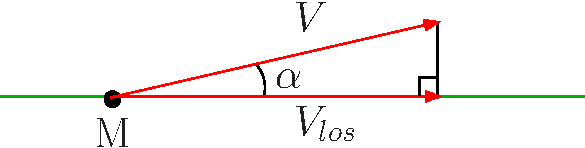
\includegraphics[width=5cm]{../figures/velproj.pdf}
\end{center}
\caption{The velocity of the cloud projected on the line-of-sight.}
\label{vproj}
\end{figure} 

 
\begin{figure}[ht]
\begin{center}
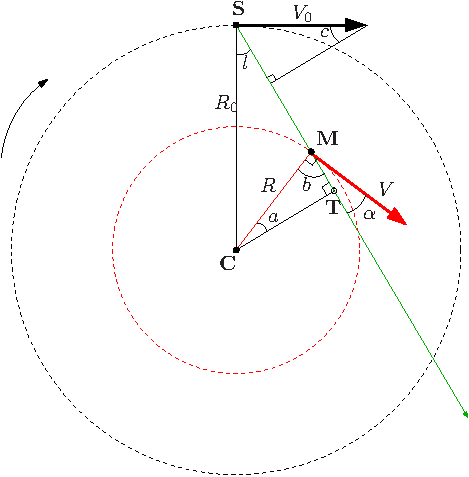
\includegraphics[width=8cm]{../figures/galgeom.pdf}
\end{center}
\caption{Geometry of the Galaxy.}
\label{galgeom}
\end{figure}  

We observe the so-called {\bf radial velocity}, 
$V_r$, the projection of the cloud's velocity on the
line-of-sight minus the velocity of the Sun on the line-of-sight. 
From Fig.~\ref{galgeom}, we obtain: 

\begin{equation}
V_r = V \cos\alpha - V_0 \sin c .
\label{eq0}
\end{equation}

In the upper triangle we see that 
$$(90-l)+90+c=180 \Rightarrow \boxed{c=l.}$$

The angle
$\alpha$ that $V$ makes with the line-of-sight can be computed from
the triangle {\bf CMT}, where we have

$$a+b+90=180 \Rightarrow b=90-a.$$

The line {\bf CM} makes a right angle with $V$. Using the above expression
for the angle $b$ (not to be confused with the Galactic latitude) we have

$$b+\alpha=90 \Rightarrow \alpha=90-b=90-(90-a)=a \Leftrightarrow \boxed{\alpha=a.}$$


The final expression for $V_r$ is obtained by rewriting eq.~\ref{eq0}:
\begin{equation}
V_r = V \cos\alpha - V_0 \sin l
\label{eq1}
\end{equation}
We now want to replace $\alpha$ with other variables. Looking at the
triangles {\bf CST} and {\bf CMT} we find that the distance between the
Galactic Center ({\bf C}) and the tangential point ({\bf T}) can be expressed in
two different ways: 
\begin{equation}
{\rm\bf CT} = R_0\sin l = R \cos\alpha
\label{eq2}
\end{equation}
Substituting $\cos \alpha$ from eq.~(\ref{eq2}) into eq.~(\ref{eq1}) we
obtain
\begin{equation}
\boxed{V_r = V \frac{R_0}{R}\sin l - V_0 \sin l .}
\label{eq3}
\end{equation}


\section{How does the gas rotate?}\label{sect-rotation}

\begin{figure}[ht]
\begin{center}
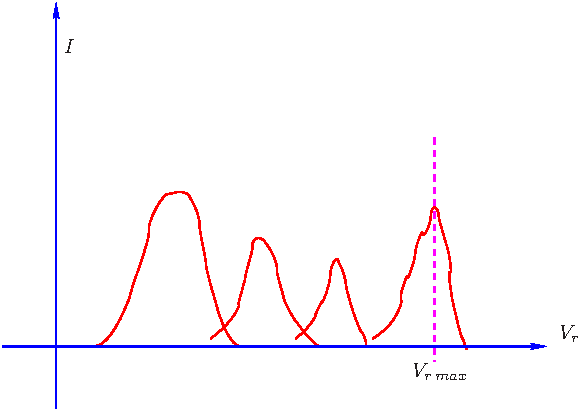
\includegraphics[width=10cm]{../figures/vmax.pdf}
\end{center}
\caption{There can be multiple velocity components in the observed spectrum.}
\label{figvmax}
\end{figure}

\begin{figure}[ht]
\begin{center}
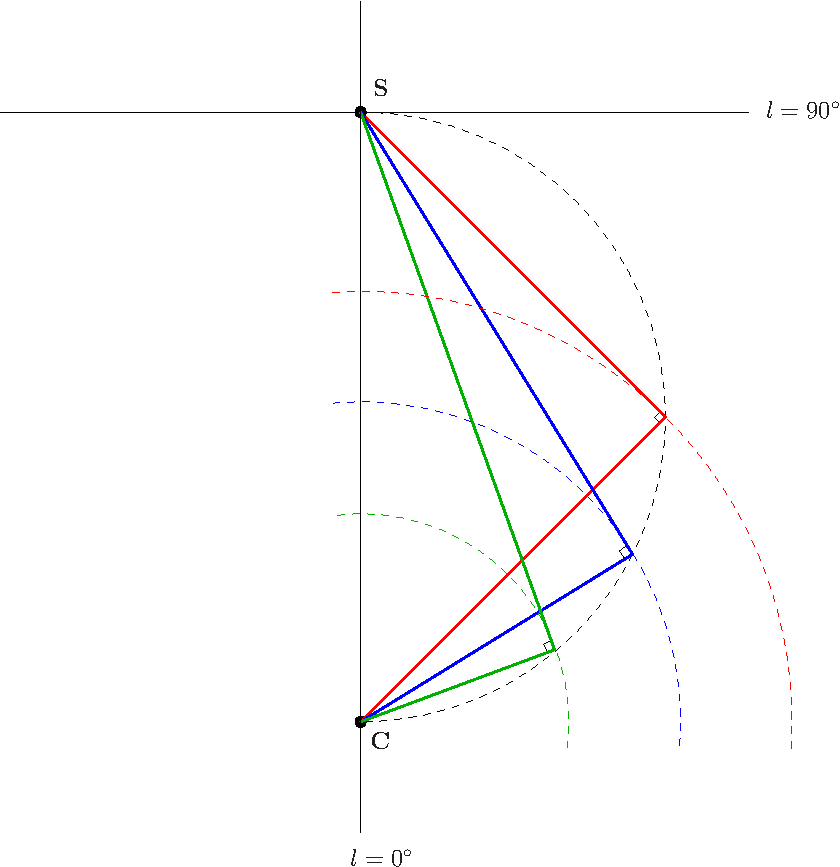
\includegraphics[width=8cm]{../figures/tangenter.pdf}
\end{center}
\caption{Interesting geometrical properties related to the tangential points. 
All tangential points lie on the half-circle centered exactly between the Sun and the Galactic center. 
The locations of three tangential points are indicated. 
Parts of some circular orbits are shown to illustrate that the velocity is at a maximum there.}
\label{tang_point}
\end{figure}
In this part of the exercise, we intend to measure the Galaxy's rotation
curve $V(R)$ in the first Galactic quadrant.

There can be several clouds along the line of sight. One usually
observes several spectral components, as illustrated on
Fig.~\ref{figvmax}.  The {\bf largest velocity component}, $V_{\rm
r,max}$, comes from the cloud {\bf at the tangential point} ({\bf T}),
where we observe the whole velocity vector along the line-of-sight. At
the tangential point, we have:
\begin{equation}
\left\{ 
\begin{array}{l}
R = R_0 \sin l \\
V = V_{r,max} + V_0 \sin l .
\end{array}
\right.
\label{eq-rv}
\end{equation}

By observing at different Galactic longitudes, we can measure
$V_{\rm r,max}$ at different values of $l$. We can then
calculate $R$ and $V$ for each $l$, and plot the rotation curve
$V(R)$.

\bigskip
{\bf Summary. } We have: 
\begin{itemize}
\item{observed HI at different Galactic longitudes $l$ in the first quadrant;}
\item{measured the maximum velocity component $V_{r,max}$ at each $l$;}
\item{assumed that the corresponding gas lies at the tangential point;}
\item{assumed that we know $R_0$ and $V_0$.}
\item{From that, we could derive the rotation curve of the Galaxy $V(R)$}. 
\end{itemize}

{\bf{$\rightarrow$}{At this point, it may be a good idea to read Appendix~\ref{app-vrot}.}}

\section{Where is the gas?}
\label{secmap}

Now we would like to find out {\em where} is the HI gas that we have detected. 
In the previous paragraph, we had used only the maximum velocity component in the spectrum, 
and assumed that it came from gas at 
the tangential point. 
Now, we shall use 
{\em all the velocity components} that we observe in the spectrum, and 
\begin{itemize}
\item{assume a certain rotation curve $V(R)$}
\end{itemize}

to infer the location of the gas. 

As in the previous paragraph, we shall 
\begin{itemize}
\item{measure $V_r$ in different directions $l$ in the Galaxy},  
\item{assume that we know $R_0$ and $V_0$.} 
\end{itemize}

Again, we use equation~\ref{eq3}. 
But, motivated by the shape our measured rotation curve (Sect.~\ref{sect-rotation}),  
we assume now that the gas in our Milky Way 
obeys {\em differential rotation}, that is, the circular velocity is
constant with radius: $V(R) = {\rm constant} = V_0$
{\bf{(Have you read Appendix~\ref{app-vrot}?)}}. 
Equation~(\ref{eq3}) thus becomes:

\begin{equation}
V_r = V_0\sin l \left( \frac{R_0}{R} -1 \right) 
\end{equation}
and we can express $R$ as a function of known quantities: 

\begin{equation}
\boxed{
R = \frac{R_0 V_0 \sin l}{V_0 \sin l + V_r} 
}
\label{Req}
\end{equation}

Now we would like to make a map of the Milky Way and place the
position of the cloud that we have detected.  From our measurement of
the radial velocity $V_r$ we have just calculated the distance of the
cloud to the Galactic center, $R$, and we know in which direction we
have observed (the Galactic longitude $l$).  


\begin{itemize}
\item{If we have observed in
Quadrant~I or Quadrant~IV, there can be {\em two possible locations} 
corresponding to given values of $l$ and $R$ (see
Figure~\ref{galgeom}): closer to us than the tangential point $T$
(the actual point {\bf M} on the figure), or farther away, at the
intersection of the {\bf ST} line and the inner circle.  }

\item{If, on the other
hand, we have observed in Quadrant~II or Quadrant~III, then the
position of the emitting gas cloud can be determined uniquely. 

{\bf{$\rightarrow$ You may want to make a drawing to convince yourself that
this is true.}} }
\end{itemize}

This can be shown mathematically: let us express {\bf SM}, 
the location of the cloud
in polar coordinates $(r,l)$, where $r$ is the distance from the sun,
and $l$ the Galactic longitude defined earlier.  In the triangle CSM,
we have the following relation:
\begin{equation}
R^2 = R_0^2 + r^2 - 2 R_0 r \cos l .
\end{equation}

This is a second-order equation in $r$, which has two possible solutions, 
$r=r_{+}$ and $r=r_{-}$:
\begin{equation}
\boxed{
r_\pm = \pm \sqrt{R^2 - R_0^2 \sin^2 l} + R_0\cos l .
}
\label{rpm}
\end{equation}

\begin{itemize}
\item{If $\cos l < 0$ (in Quadrant~II or III), one can show that
there is one and only one positive solution, $r_+$, because $R$ is
always larger than $R_0$.}

\item{In the other quadrants, there can be two
positive solutions.}
\end{itemize}

Negative values of $r$ should be discarded because  
they have no physical meaning.  If one obtains two positive
solutions, one should observe toward the same Galactic longitude but
at different Galactic latitudes to determine which solution is
correct.  By observing at a higher Galactic latitude, one wouldn't be able 
to see a distant cloud lying in the Galactic plane.


\section{Estimating the mass of our Galaxy}

Assuming that most of the mass of our Galaxy is distributed in 
a spherical component around the center 
(in the so-called dark matter halo), one can calculate the
mass $M(<R)$ enclosed within a given radius $R$. 
Indeed, for a spherically symmetric distribution, a theorem
by Jeans tells us that the mass outside a radius $R$ doesn't
affect the velocity of a point at that radius. 
Also, thanks to another theorem also due to Jeans, 
the matter at radius $R$ moves in the same way as if all the
mass were located in the center. 
Note that this is true only in the case of a spherically symmetric
distribution!
Then we can write (see also Appendix~\ref{app-vrot})
\begin{equation}
\frac{V^2}{R}= \frac{GM(< R)}{R^2}
\end{equation}
where $G$ is the gravitational constant. 
We can derive $M(< R)$: 
\begin{equation}
\boxed{M(<R) =  \frac{V^2 R}{G}. }
\end{equation}

{\bf{$\rightarrow$ Taking $R = 10$~kpc, $V= V_\odot = 220$~km/s, 
calculate the mass enclosed within 10~kpc.  Express the mass in 
kg and in solar masses. }}

\bigskip
$G = 6.67 \cdot 10^{-11}$ ~N m$^2$ kg$^{-2}$

1 M$_\odot = 2 \cdot 10^{30}$~kg

1 kpc = 10$^3$ pc; 1 pc $= 3.086\cdot 10^{16}$ m

